
\section{Application 1: Expression Flow for 3D-Aware Face
Component Transfer}
We now introduce one application of face fitting. The goal of this application is to transfer the mouth from one to another. We first introduce the pipeline of this project and then introduce each components in more detail.
\begin{figure}[H]
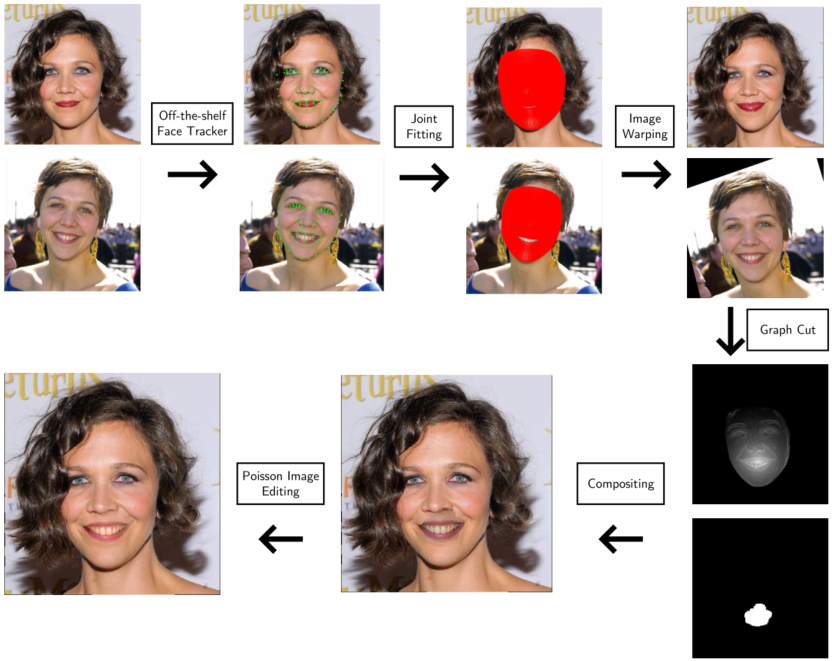
\includegraphics[width=\textwidth]{./img/expression-flow-pipeline}
\caption{Step 1: use the off-the-shelf face tracker to get the 2D face landmarks. \\
Step 2: Perform joint face fitting on the two face images. \\
Step 3: Perform image warping to align the two images for later image compositing. \\
Step 4: Generate prior map and perform graph cut to find the best seam. \\
Step 5: Sometimes there will be visible artifact on the border, we do one step of Poisson image edting on the composited image.}
\end{figure}

\subsection{Joint fitting of the model}
In some scenerios where we want to fit models for the same person that appeared in multiple images at the same time. We will need to fit the same identity weights $\mathbf{w}^{\text{id}}$ and fit the expression weights $\mathbf{w}^{\text{expr}}$ for different images. We adapt the previous algorithm as follows.

\subsection{Finding the best seam}
We can formulate this into a graph cut problem. In a graph cut framework. We first specify the data cost 
$$C(p) = \alpha \exp(-\frac{D_s(p)}{\sigma_d}) + (1 - \alpha) \left(1 - \exp(-\frac{||\nabla S(p)||}{\sigma_s})\right)$$
where $D_s(p)$ is the spatial distance from $p$ to the nearest pixel selected by the user, $||\nabla S(p)||$ is the gradient magnitude at $p$, and $\sigma_d$, $\sigma_s$ and $\alpha$ are parameters controlling the shape and weight of each term. $L(p)$ is the label of $p$. The data penalty in the graph cuts formulation is then defined as $C_d(p, L(p)) = 1 - C(p)$ is $L(p) = 1$(inside the crop region), and $C_d(p, L(p)) = C(p)$ if $L(p) = 0$(outside the crop region). 

Then we specify the smooth cost in the "match gradient" formulation for setting the neighborhood penalty $C_i(p, q, L(p), L(q))$ as:
$$||\nabla S_{L(p)}(p) - \nabla S_{L(p)}(p)|| + ||\nabla S_{L(p)}(q) - \nabla S_{L(q)}(q)||$$
This formulation encourages the cut to happen at the place where the difference of the gradients is small.


\subsection{Poisson Image Editing}
Here we introduce poisson image editing as a technique to remove visual seams. Visual seams occur because of the color mismatch between the two images. In poisson image editing we fix the colors of the boundary (taken from the background image) and provides a vector field that defines the structure of the image to be copied (taken from the foreground). The result image is generated by minimizing the squared error terms between the gradient of the result image and the guidance vector field.

The basic idea is to preserve the laplacian of the image while keep the boundary fixed.
$$\int_\Omega ||\Delta(\mathbf{x}_{1} - \hat{\mathbf{x}})||^2 \; d\mathbf{A} \quad \text{subject to } \hat{\mathbf{x}}^{\text{boundary}} = \mathbf{x}^{\text{boundary}}_2$$
Where the $\hat{\mathbf{x}}$ is the pixel value of inner part to be determined, $\mathbf{x}_1$ is the foreground image, $\mathbf{x}_2$ is the background image. 


\subsection{Results}
\begin{figure}[H]
    \centering
    \subfloat[]{\includegraphics[width=0.33\textwidth]{./img/flow2/img1}}
    \hfill
    \subfloat[]{\includegraphics[width=0.33\textwidth]{./img/flow2/img2}}
    \hfill
    \subfloat[]{\includegraphics[width=0.33\textwidth]{./img/flow2/blend_img}}
\end{figure}

\begin{figure}[H]
    \centering
    \subfloat[]{\includegraphics[width=0.33\textwidth]{./img/flow3/img1}}
    \hfill
    \subfloat[]{\includegraphics[width=0.33\textwidth]{./img/flow3/img2}}
    \hfill
    \subfloat[]{\includegraphics[width=0.33\textwidth]{./img/flow3/blend_img}}
\end{figure}

Here for each triple of images, we use the first image as the background image, the second as foreground image. Using the techniques described above, we get the third image as the result.
